\documentclass[tikz,border=12pt]{standalone}
\usepackage{amsmath,amssymb}
\usetikzlibrary{calc,arrows.meta}

\begin{document}
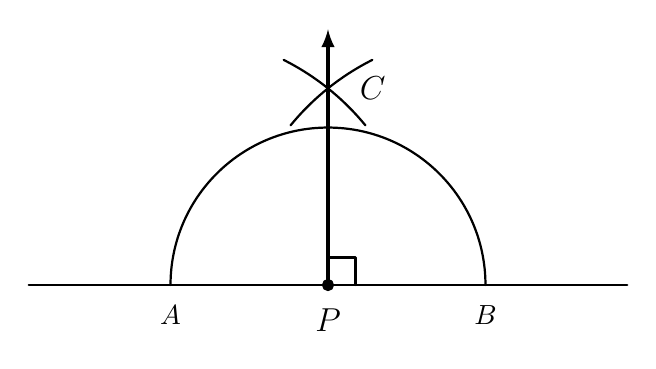
\begin{tikzpicture}[>=latex, line cap=round, line join=round]
  % Parameters
  \def\r{2.0}     % Radius of base semicircle from P
  \def\R{3.2}     % Radius of crossing arcs
  
  % Baseline
  \draw[thick] (-3.8, 0) -- (3.8, 0);

  % Given point P on baseline
  \coordinate (P) at (0, 0);
  \filldraw[black] (P) circle (2pt) node[below=5pt, font=\large\bfseries] {$P$};

  % Semicircle centered at P cutting baseline at A and B
  \draw[thick] (\r, 0) arc (0:180:\r);
  
  \coordinate (A) at (-\r, 0);
  \coordinate (B) at (\r, 0);
  \node[below=4pt, font=\normalsize] at (A) {$A$};
  \node[below=4pt, font=\normalsize] at (B) {$B$};

  % Crossing arcs from A and B above P
  \pgfmathsetmacro{\yint}{sqrt(\R*\R - \r*\r)}
  \pgfmathsetmacro{\angA}{atan2(\yint, \r)}
  \pgfmathsetmacro{\angB}{180 - \angA}

  \draw[thick] ($(A) + ({\angA - 12}:\R)$) arc ({\angA - 12}:{\angA + 12}:\R);
  \draw[thick] ($(B) + ({\angB - 12}:\R)$) arc ({\angB - 12}:{\angB + 12}:\R);

  \coordinate (C) at (0, \yint);
  \node[right=8pt, font=\large] at (C) {$C$};

  % Perpendicular ray from P through C
  \draw[very thick, ->] (P) -- (0, {\yint * 1.3});

  % Right angle indicator at P
  \draw[thick] (0, 0.35) -- (0.35, 0.35) -- (0.35, 0);

\end{tikzpicture}
\end{document}
